\documentclass{exam}
\usepackage{graphicx} 


%Format Header and footer
\pagestyle{headandfoot}
\header{\footnotesize Klass:\\Namn:}{\Large\textbf{Evolution}}{\footnotesize  BIOBIO01 - 2024\\Viktor Arohlén}
\headrule
\footrule
\setlength{\columnsep}{0.25cm}
%\setlength{\columnseprule}{1pt}
\footer{}{Sida \thepage}{}
%\extrafootheight{-2cm}

\begin{document}
\vspace{5mm} %5mm vertical space
\begin{center}
\fbox{\fbox{\parbox{6in}{\centering
\textbf{Grundläggande frågor}: svara kortfattat (bedöms på E- till C-nivå)
}}}
\end{center}
\vspace{5mm} %5mm vertical space
\begin{questions}
\question Förklara följande begrepp

\begin{itemize}
  \item Mutation 
  \vspace{10mm}
  \item Naturligt urval
  \vspace{10mm}
  \item Selektionstryck
  \vspace{10mm}
  \item Hybridisering
\end{itemize}
\vspace{10mm} %5mm vertical space
\question
Förklara vad en korsningsbarriär mellan arter är och ge två olika exempel på sådana barriärer?
\vspace{30mm} 
\question
Om vi vill studera evolutionen, vilka arter bör vi studera? Motivera!
\vspace{30mm} 
\question
Vilket av följande begrepp beskriver situationen där en fjärils färgmorf (färgvariant) är mer attraktiv för en partner, vilket leder till att färgmorfen blir vanligare i populationen?
\vspace{5mm}
\begin{checkboxes}
    \choice sexuell selektion
    \choice genetisk drift
    \choice flaskhalseffekt
    \choice naturligt urval
\end{checkboxes}
\break
\question 
Vilket av följande alternativ förklarar bäst begreppet samevolution?
\vspace{5mm}
\begin{checkboxes}
\choice En egenskap hos en art förs vidare trots att den egentligen inte fyller någon funktion.

\choice Liknande egenskaper hos arter som inte har en gemensam föregångare (förfader) som har denna egenskap.

\choice En art utvecklar på nytt en egenskap som försvunnit i ett tidigare skeda av artens evolution.

\choice En arts egenskaper utvecklas i samspel med en annan art.
\end{checkboxes}

\vspace{10mm}
\question
Vilket typ av urval visualiserar grafen nedan? Ge ett exempel på när ett sådant urval sker

\begin{figure}[h]
    \centering
    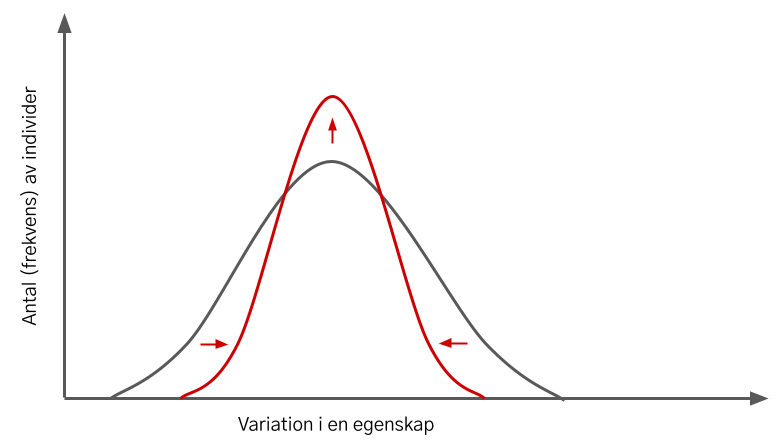
\includegraphics[width=0.7\linewidth]{06f57399-163d-4981-a6b3-9370f8174f29.png}
\end{figure}
\break
\vspace{5mm} %5mm vertical space
\begin{center}
\fbox{\fbox{\parbox{6in}{\centering
\textbf{Fördjupande frågor}: svara mer utförligt (bedöms på E- till A-nivå)
}}}
\end{center}
\question 
Tänk dig att en hane och en hona av en viss fågelart blåser iland på en avlägsen ö. På ön kommer de att bli stamfäder till en ny population.

Resonera om hur den nya populationen på ön kommer att utvecklas jämfört med den gamla på fastlandet.
\vspace{60mm}
\question
En stor problematik idag är multiresistenta bakterier, det vill säga bakterier som är okänsliga för flera olika sorters antibiotika. För hundra år sedan existerade knappt sådana bakterier. Förklara med hjälp av naturvetenskapliga evolutionära begrepp hur problematiken har utvecklas.

\break
\question
Evolutionsteorin är sedan länge den teori som världens biologer arbetar efter och räknas i dag till en av de stora, etablerade naturvetenskapliga teorierna.

Under de senaste åren har den utmanats av teorin om intelligent design (ID). Förespråkarna för ID hävdar att evolutionsteorin är otillräcklig och att det bara går att förklara organismernas mångfald och livets alla komplexa former som orsakade av en intelligent ”designer” (som skulle kunna vara Gud).

Hur skulle du, som biolog, argumentera \textbf{för} evolutionsteorin \textbf{mot } en ID-förespråkare, som säger att evolutionsteorin är en bluff?



\end{document}
